\documentclass[conference]{IEEEtran}

\usepackage{pythonhighlight}
% \documentclass{article}
\usepackage{array}
\usepackage{graphicx}
\usepackage{subcaption} 
\usepackage{graphicx}
\usepackage{hyperref}
\usepackage{float}
\usepackage[english]{babel}
\usepackage{listings} % code blocks
\usepackage[utf8]{inputenc}
\usepackage{amsmath}
\usepackage[acronym]{glossaries}
\usepackage{fancyhdr}
\usepackage{lastpage}
\makeglossaries
%\usepackage{etoolbox} % citações

\pagestyle{fancy}
\fancyhf{}
\fancyfoot[C]{Page \thepage\ of \pageref{LastPage}}

\hyphenation{}

\begin{document}
% paper title
% can use linebreaks \\ within to get better formatting as desired
\title{Analysis and Forecasting of Monthly Electricity Consumption in France}

% author names and affiliations
% use a multiple column layout for up to three different
% affiliations
\author{
    \IEEEauthorblockN{Cristiano Nicolau}
   \IEEEauthorblockA{
        Séries Temporais 24/25\\
        Departamento de Matemática\\
        Universidade de Aveiro\\
        Aveiro, Portugal\\
        cristianonicolau@ua.pt
    }
    \and
    \IEEEauthorblockN{Maria Abrunhosa}
   \IEEEauthorblockA{
        Séries Temporais 24/25\\
        Departamento de Matemática\\
        Universidade de Aveiro\\
        Aveiro, Portugal\\
        maria.abrunhosa@ua.pt
    }
}
% make the title area
\maketitle

\begin{abstract}
This study focuses on the analysis and forecasting of monthly electricity consumption in France, utilizing Eurostat data from 2008 to 2025. To achieve this, we compared several statistical time series models, specifically SARIMA, ETS, and STLM.
Our evaluation revealed that the manually parameterized SARIMA model exhibited the lowest values for information criteria (AIC, AICc, and BIC), indicating a better balance between model fit and complexity. However, the SARIMA model with automatic parameter selection stood out due to its superior predictive capability on the test set, demonstrating the lowest errors (RMSE, MAE, MAPE, and Theil's U). In contrast, the ETS and STLM\_ARIMA models showed inferior performance in both evaluations.
\end{abstract}

\begin{center}
    \textit{\textbf{Keywords} — Electricity Consumption Analysis and Forecasting, Time Series Analysis, Forecasting, ARIMA, SARIMA, ETS, STLM}
\end{center}
\IEEEpeerreviewmaketitle
%\acrlong{da}
%\acrshort{da}
%\acrfull{da}

\newacronym{acf}{ACF}{Autocorrelation Function}
\newacronym{pacf}{PACF}{Partial Autocorrelation Function}

\newacronym{adf}{ADF}{Augmented Dickey-Fuller Test}
\newacronym{kpss}{KPSS}{Kwiatkowski-Phillips-Schmidt-Shin Test}
\newacronym{ljung}{Ljung-Box}{Ljung-Box Test for Autocorrelation}
\newacronym{arch}{ARCH}{Autoregressive Conditional Heteroskedasticity Test}

\newacronym{arima}{ARIMA}{AutoRegressive Integrated Moving Average}
\newacronym{sarima}{SARIMA}{Seasonal AutoRegressive Integrated Moving Average}
\newacronym{ets}{ETS}{Error, Trend and Seasonality}
\newacronym{stl}{STL}{Seasonal-Trend decomposition using Loess}
\newacronym{stlm}{STLM}{STL decomposition followed by ARIMA}

\newacronym{aic}{AIC}{Akaike Information Criterion}
\newacronym{aicc}{AICc}{Corrected Akaike Information Criterion}
\newacronym{bic}{BIC}{Bayesian Information Criterion}

\newacronym{mae}{MAE}{Mean Absolute Error}
\newacronym{mse}{MSE}{Mean Squared Error}
\newacronym{rmse}{RMSE}{Root Mean Squared Error}
\newacronym{mape}{MAPE}{Mean Absolute Percentage Error}
\newacronym{smape}{sMAPE}{Symmetric Mean Absolute Percentage Error}
\newacronym{me}{ME}{Mean Error}

\newacronym{garch}{GARCH}{Generalized Autoregressive Conditional Heteroskedasticity}

\newacronym{loess}{LOESS}{Locally Estimated Scatterplot Smoothing}

\section{Introduction}

Electricity consumption is a crucial indicator of a country's economic and social well-being, reflecting not only industrial and commercial activity but also the population's living standards. Understanding and forecasting it are fundamental for energy planning, infrastructure management, and the development of sustainability policies. In a global scenario of growing concern over climate change and energy transition, the ability to accurately predict electricity demand becomes even more relevant. Accurate forecasts allow for optimizing energy generation and distribution, preventing grid overloads, and anticipating future needs, contributing to the security and efficiency of electrical systems.\\

This study is dedicated to the analysis and forecasting of monthly electricity consumption in France, a country with one of Europe's largest economies and a complex and diverse energy sector, characterized by a strong reliance on nuclear power (84.7\%) and increasing investment in renewable energies \cite{EDF2012}. To this end, we will use a time series, compiled by Eurostat, covering monthly energy consumption in France from 2008 to 2025 \cite{EurostatElectricityConsumption}. The main objective is to identify the most suitable statistical time series models for capturing underlying energy consumption patterns and generating reliable forecasts. Data analysis will include identifying trends, seasonalities, and any anomalies that may influence electricity consumption, providing a deeper understanding of the time series.
\section{Data and Exploratory Analysis}

Before modeling the data, we did an exploratory data analysis that is an initial visualization and decomposition of the data to understand its underlying structure, including trend and seasonality. We also divided the data into training and testing sets.
After that, we applied some data transformation to stabilize the variance and stationarize the series.\

\subsection{Dataset Description}
The analysed data was obtained from the Eurostat portal \cite{EurostatElectricityConsumption}. The dataset refers to the monthly amount of electricity available on the domestic market in France, expressed in gigawatt hours (GWh).
The data is updated monthly and covers the period from January 2008 to March 2025, comprising 207 months of observations.
The selected indicator is 'Electricity available for the internal market – monthly data (France)'.

This type of series is particularly relevant for studying energy consumption patterns over time, including seasonal variations and structural trends.

The dataset was imported from a .csv file to create a time series object with a monthly frequency starting in January 2008.

\subsection{Separation into training and testing sets}

To properly assess the models' predictive capacity, the data was divided as follows:

- Training: 80\% of the initial observations (January 2008 – October 2021), 165 observations.

- Test: the remaining 20\% (November 2021 – March 2025), 42 observations.

We only applied transformations to the training set (repeating this process in the test set when necessary) to avoid data leakage.

\subsection{Exploratory Analysis}

To study the existence of outliers, we used a box plot, Fig.\ref{fig:bx-plot}, treating the numerical values by replacing commas with decimal points. We observed that the boxplot indicates the absence of outliers.

\begin{figure}[H]
    \centering
    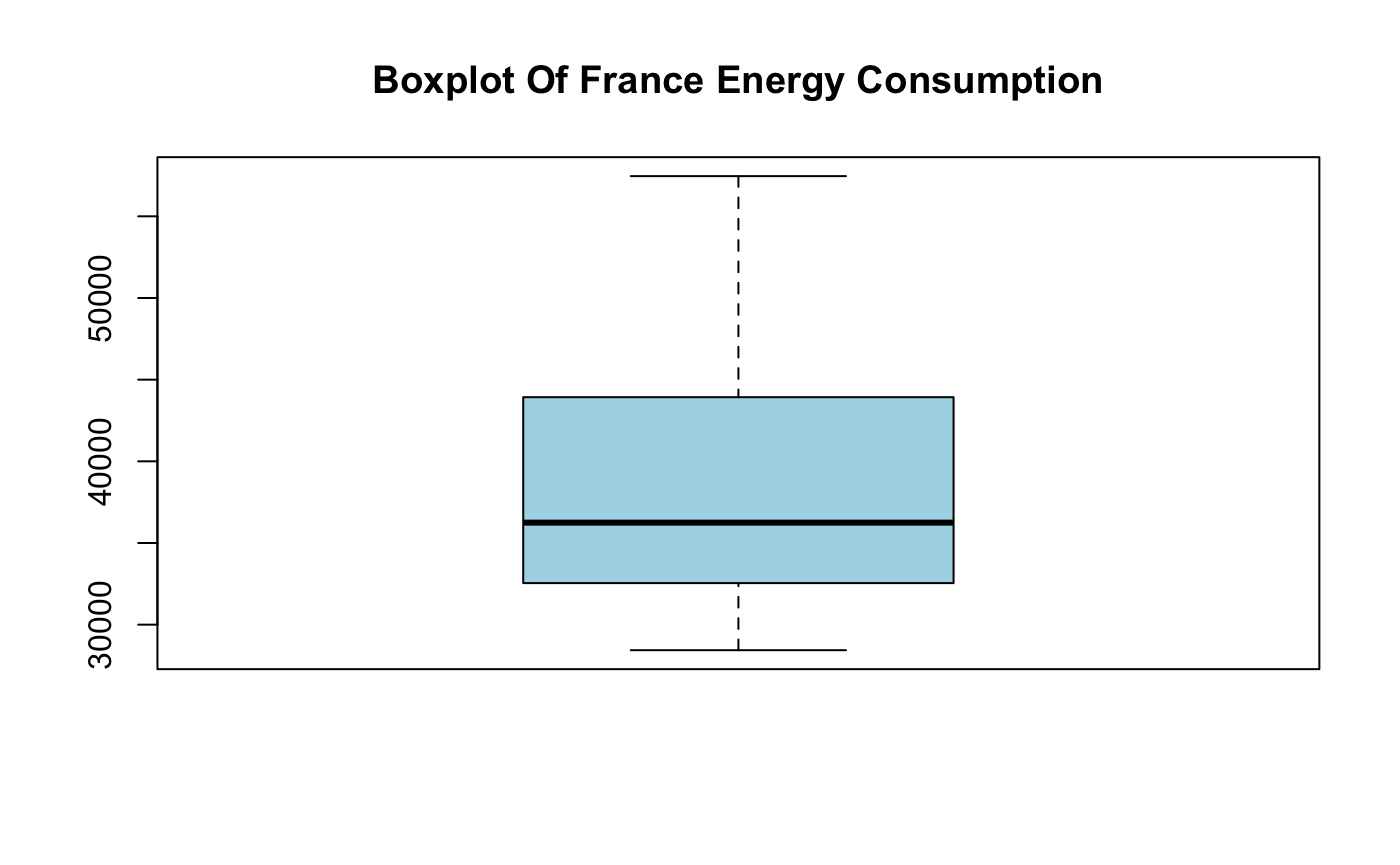
\includegraphics[width=0.75\linewidth]{images/box-plot.png}
    \caption{Box-Plot of Energy Consumption in France}
    \label{fig:bx-plot}
\end{figure}

To identify visual patterns we visualizes the time series using a plot, Fig\ref{fig:f-plot}. 
\begin{figure}[H]
    \centering
    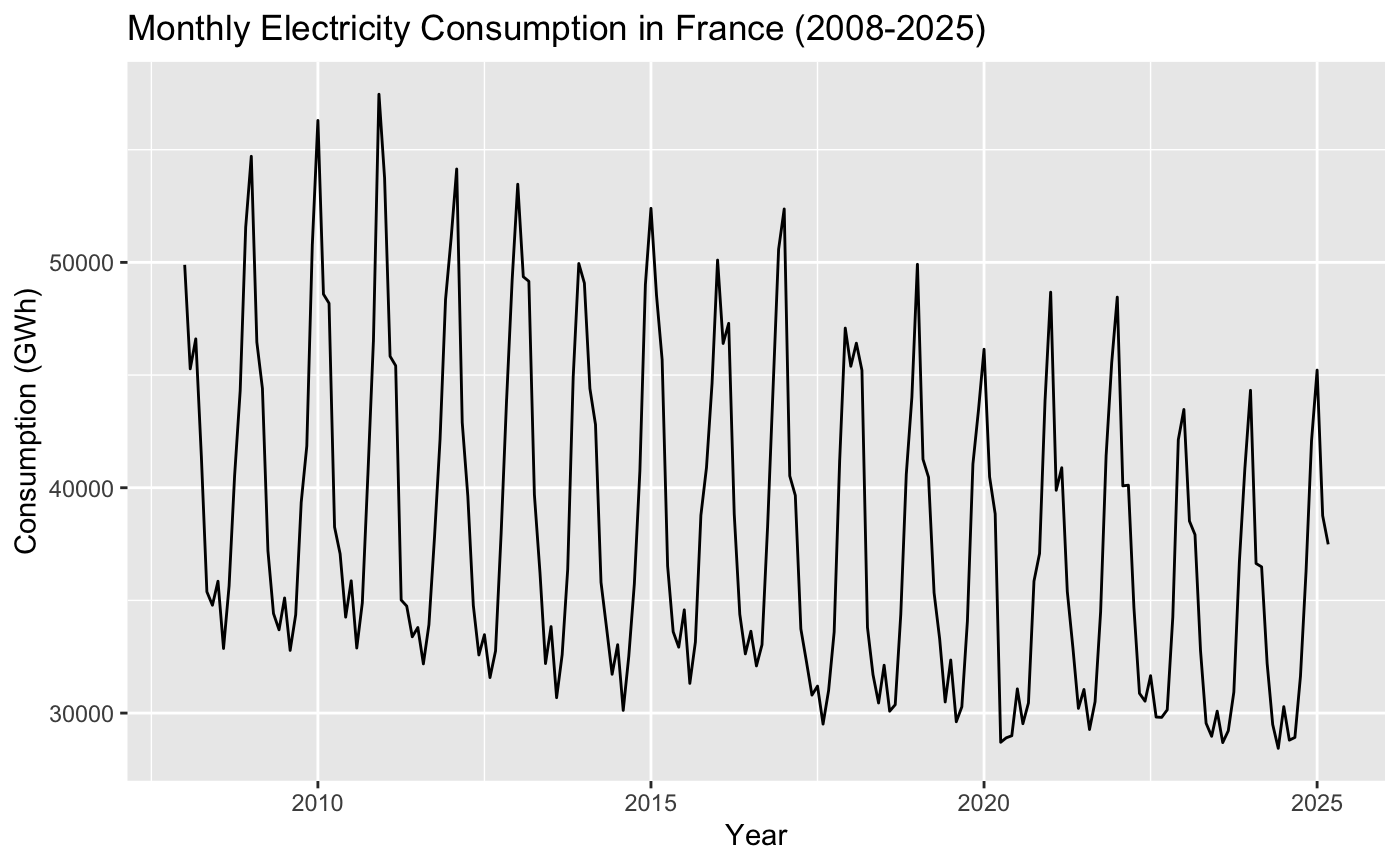
\includegraphics[width=0.75\linewidth]{images/f-plot.png}
    \caption{Monthly Electricity Consumption in France (2008-2025)}
    \label{fig:f-plot}
\end{figure}
We concluded that the time series has:
\begin{itemize}
    \item Strong seasonality: there are regular peaks in the winter months and lows in the summer months.
    \item Slightly decreasing trend: especially since 2010.
    \item Slight variation in variance: the level of consumption shows greater variability in the early years, which seems to decrease slightly over time.
\end{itemize}

\vspace{0.5\baselineskip}


We also decomposed the time series to better visualize these components (trend, seasonality and noise) and prove our last conclusions, Fig.\ref{fig:f2}.
We applied classical decomposition since our data has clear and stable trend and sazonality.

The decomposition confirms the strong seasonal pattern and a visible, though slightly noisy, trend that becomes evident especially after 2010.

\begin{figure}[H]
    \centering
    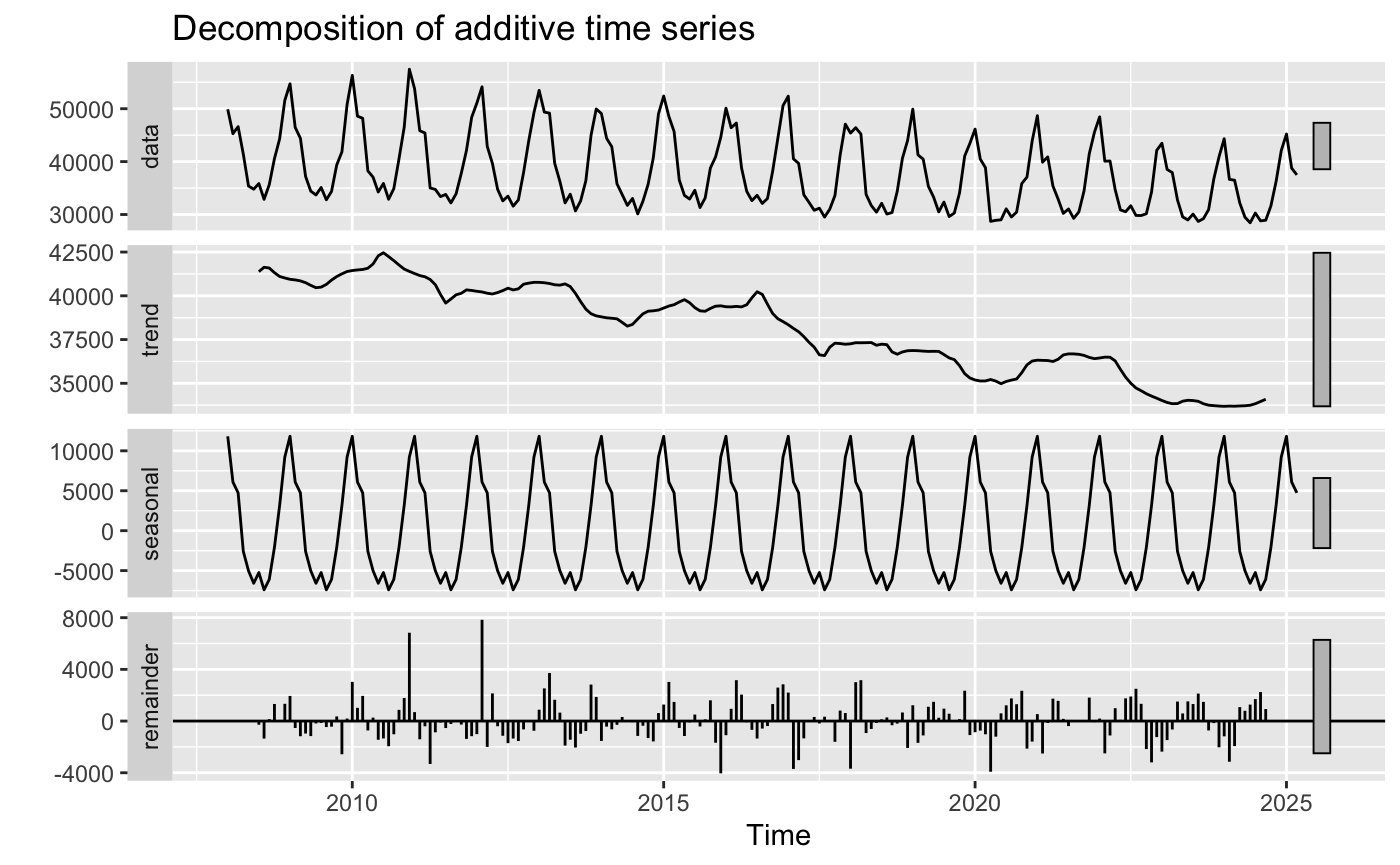
\includegraphics[width=1\linewidth]{images/f2.png}
    \caption{Time Series Decomposition}
    \label{fig:f2}
\end{figure}

The characteristics of the series, seasonality and trend, suggest the need for models such as SARIMA, ETS or STL + ARIMA decomposition, that will be explored in the following sections.

\subsection{Data Transformations}
Following the initial exploratory analysis, we confirmed that the time series exhibited variations in variance and trend fluctuations. To address this, we need to apply some transformations.

\subsubsection{Stabilise Variance}

\vspace{0.5\baselineskip}

To stabilise the variance of the time series, we applied a logarithmic transformation, Fig.\ref{fig:log}
A visual inspection of the original series indicates greater seasonal fluctuations during periods of higher consumption, notably between 2008 and 2012, and less pronounced variation in subsequent years.
This pattern indicates that the variance is not constant and may depend on the level of the series, a condition known as heteroscedasticity.

Applying the log() transformation reduces this heteroscedasticity, making the series more suitable for modelling, particularly for models that assume constant variance.

\begin{figure}[H]
    \centering
    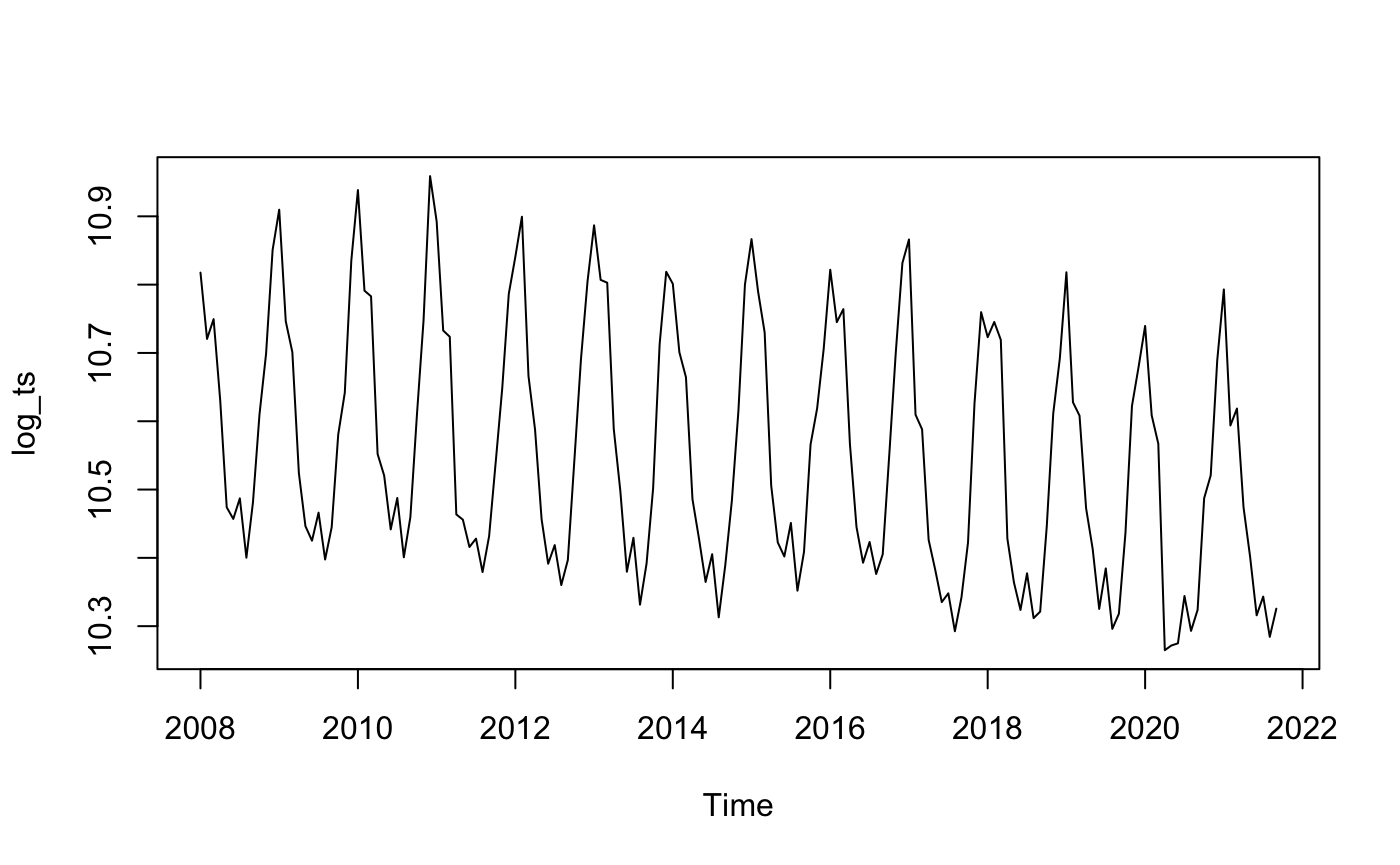
\includegraphics[width=0.9\linewidth]{images/log.png}
    \caption{Time Series Log Transformation}
    \label{fig:log}
\end{figure}


\subsubsection{Stationarity Testing and Differencing}

\vspace{0.5\baselineskip}

For the conclusions of the exploratory analysis we already known that the trend was not constant just by observing the time series plot. However, to rich this paper, we did some formal stationarity tests with ADF and KPSS to check if we do need to differenciate the time series. We can confirm this with statistical tests.

We applied two complementary tests:
\begin{itemize}
    \item Augmented Dickey-Fuller (ADF) test:
    \begin{center}
        \( H_0: \text{The series is non-stationary (has a unit root).} \)
    \end{center}
    \item KPSS test:
    \begin{center}
        \( H_0: \text{The series is stationary.} \)
    \end{center}
\end{itemize}

\vspace{0.5\baselineskip}

For both tests, a low p-value (less than 0.05) means that we can reject the null hypothesis (H0).
However, as the results were ambiguous, it is safer to differentiate the series, assuming that it is not yet fully stationary.

\vspace{0.5\baselineskip}

To determine the order of differencing we used the functions \textit{ndiffs()} for regular differencing and \textit{nsdiffs()} for seasonal differencing. The results were 1 for each differencing.

\begin{figure}[H]
    \centering
    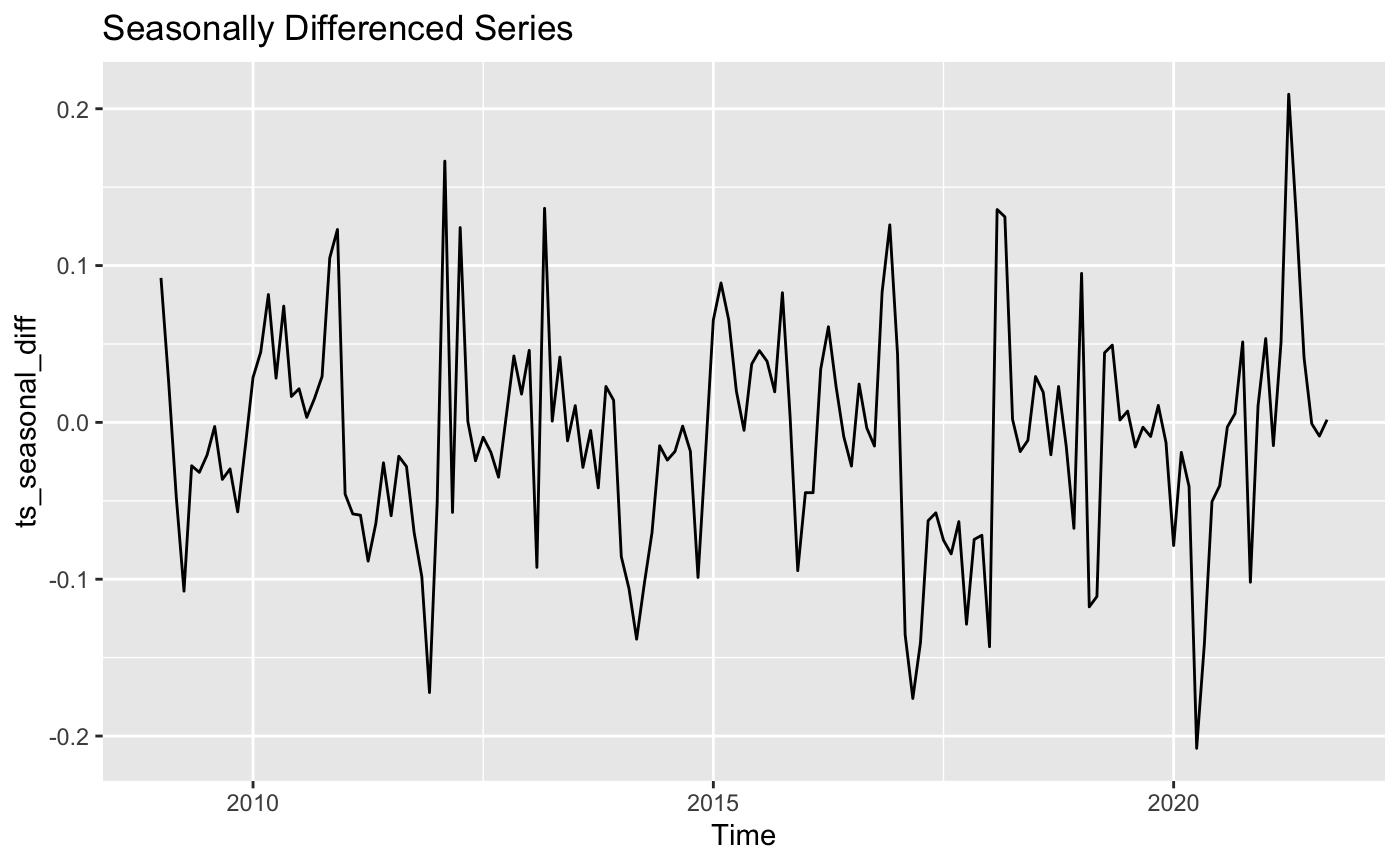
\includegraphics[width=0.9\linewidth]{images/seasonali_diff.png}
    \caption{Seasonally Differenced Series ((D=1)}
    \label{fig:seasonali_diff}
\end{figure}

For this reason, we started with seasonal differencing, Fig.\ref{fig:seasonali_diff}, (lag = 12) due to the strong 12-month seasonality.
Although the seasonal pattern has now disappeared, there may still be a trend present, so we applied a regular first difference to remove any remaining trend, Fig.\ref{fig:seasonaly_regulary}.

\begin{figure}[H]
    \centering
    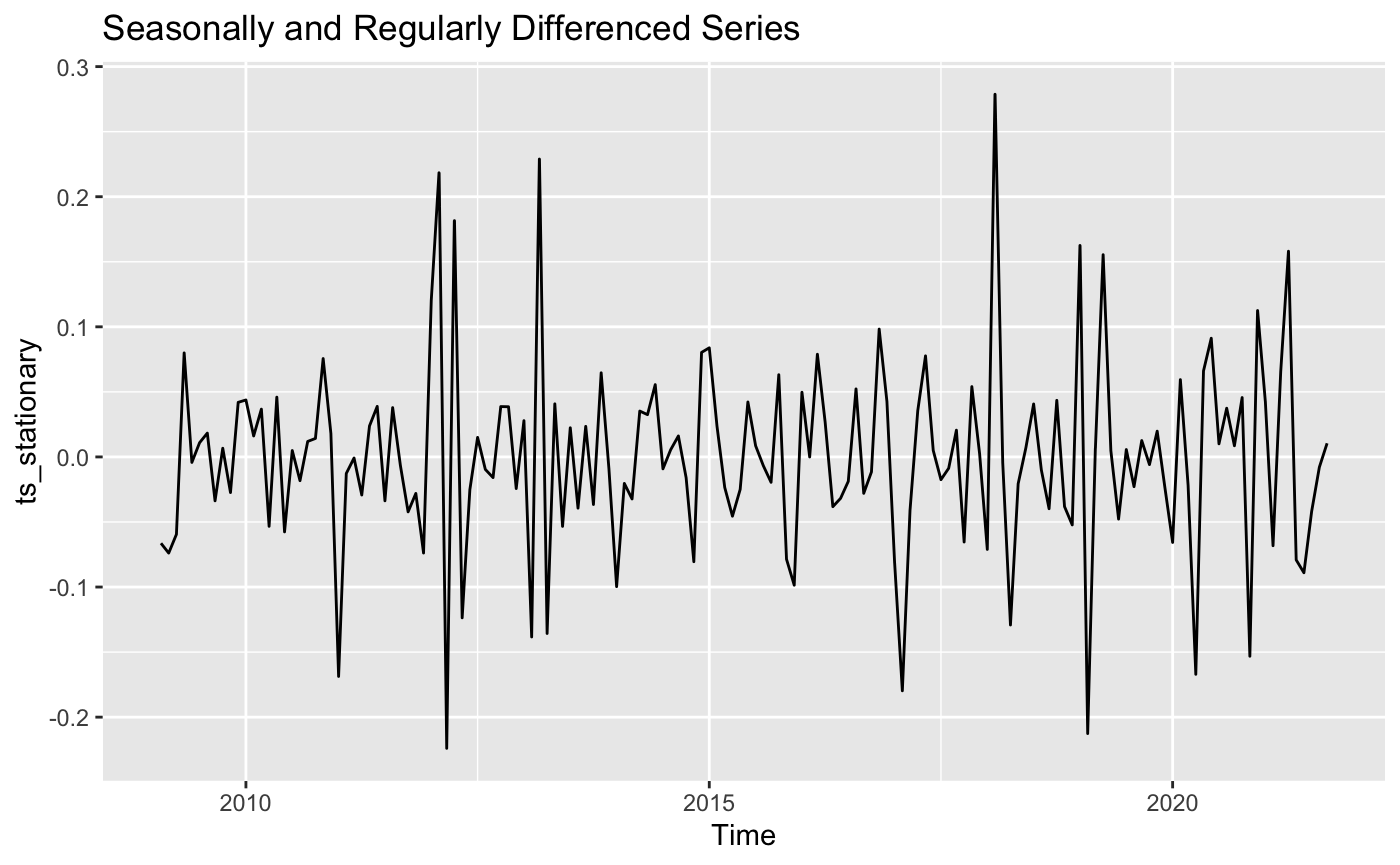
\includegraphics[width=0.9\linewidth]{images/seasonaly_regulary.png}
    \caption{Seasonally and Regularly Differenced Series(d=1)}
    \label{fig:seasonaly_regulary}
\end{figure}


To confirm the stationarity of the time series after differencing, we re-ran the stationarity tests (ADF and KPSS). Both tests then agreed on the stationarity of the time series. The Augmented Dickey-Fuller (ADF) test strongly rejected the null hypothesis of non-stationarity ($p < 0.01$), while the KPSS test failed to reject the null hypothesis of stationarity ($p > 0.1$). These results confirmed that the differenced series was stationary.
\section{Model Proposals}

In this section, we use the Box–Jenkins methodology to develop and assess SARIMA models for log-transformed and differenced time series data.
Then, we evaluated the residuals for white noise behaviour, checking for autocorrelation and verifying the statistical significance of the model coefficients.
This rigorous process ensures that the chosen model is statistically valid and suitable for forecasting.\\

To rigorously compare different modeling methodologies, we developed multiple candidate models based on the transformed and stationary series. Given the complexity and structure of the time series, specifically the presence of seasonality, a slight trend, and possibly varying variance, it is essential to explore alternative approaches.\\

The primary objective of this project is to evaluate the effectiveness of each model type in both the training and forecasting phases. To that end, we compare the model fit criteria and diagnostics in this section (Section 3), and evaluate predictive performance metrics in Section 4. This allows us to strike a balance between in-sample accuracy and out-of-sample generalization, while avoiding overfitting.

Since the models will later be used for forecasting, we previously split the dataset into training and test sets. All models are trained exclusively on the training set to prevent data leakage. 

\subsection{Box-Jenkins Methodology}
Our modelling approach is based on the Box-Jenkins methodology, which is specifically designed for ARIMA and SARIMA models. This methodology consists of four iterative steps:

\begin{enumerate}
    \item Model identification: analysing the ACF and PACF plots, along with stationarity tests (ADF and KPSS) to determine the appropriate model orders.
    \item Parameter estimation: fitting the model to the training data and estimating its parameters using likelihood-based methods.
    
    \item Diagnostic checking: validating the model's adequacy by analysing the residuals through autocorrelation checks, white noise behaviour and the Ljung–Box test.

    \item Forecasting: using the selected model to produce forecasts and assess their accuracy against a test set.
\end{enumerate}

These steps were rigorously applied to the SARIMA models developed in this project, both via automated selection with \textit{auto.arima()} and through manual specification. In parallel, we compared this approach with two alternative methods: STLM decomposition followed by ARIMA and exponential smoothing (ETS). This allowed us to evaluate different strategies for capturing the underlying structure of the series.

\subsection{Analysis of ACF and PACF for model identification}

To identify the appropriate orders of an ARIMA model, it is essential to analyse the autocorrelation function (ACF) and the partial autocorrelation function (PACF). These tools are fundamental to time series analysis and were only applied after the series has been transformed to achieve stationarity, through logarithmic transformation and differencing.

\begin{itemize}
    \item ACF (Autocorrelation Function): It measures the correlation between the time series and its own lagged values. It is particularly useful for identifying the order of the moving average component (q).

    \item PACF (Partial Autocorrelation Function): Measures the correlation between the time series and its lags while controlling for other lags. It is typically used to determine the autoregressive order (p).
\end{itemize}

\begin{figure}[H]
    \centering
    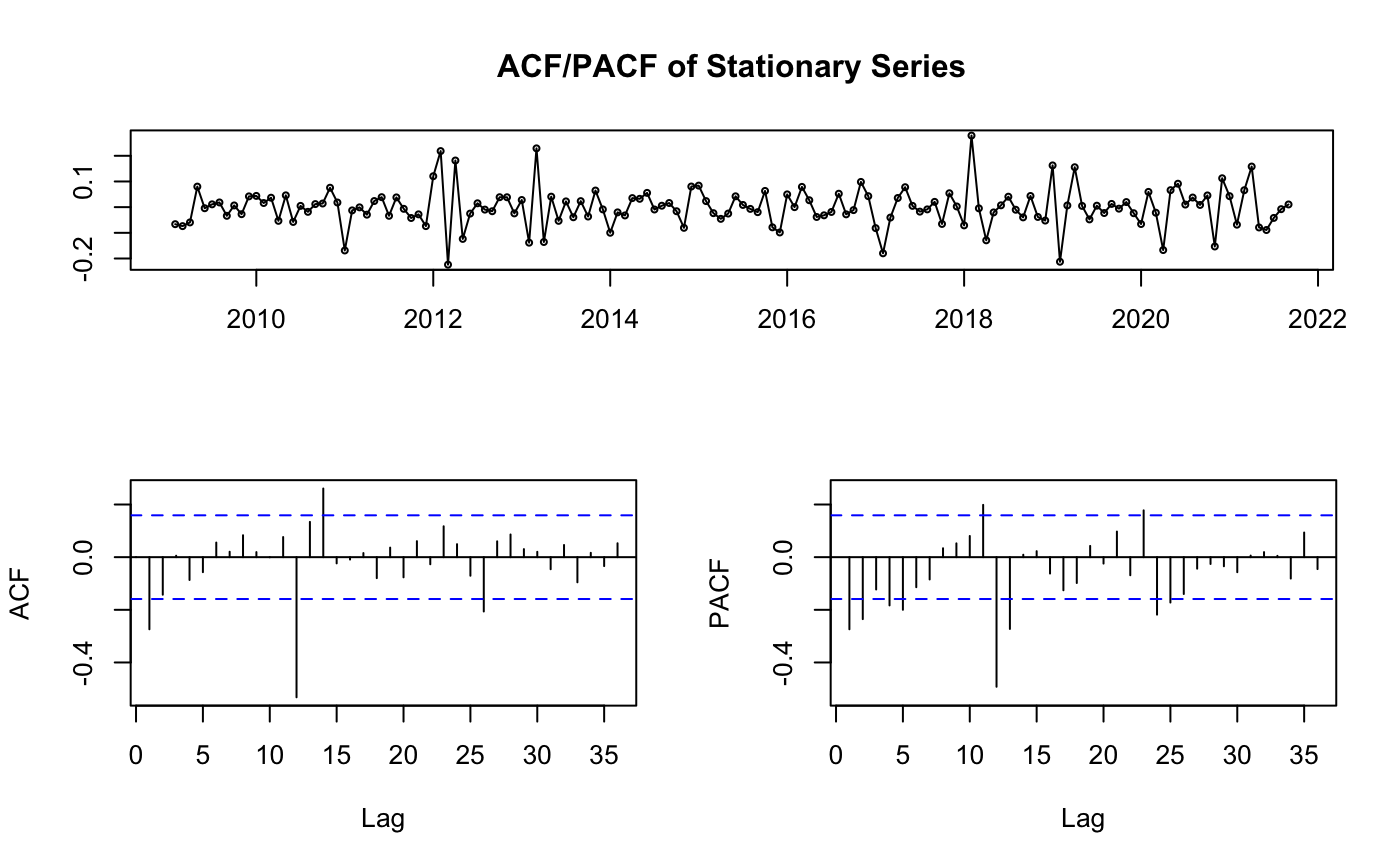
\includegraphics[width=1\linewidth]{images/ACF_PAC.png}
    \caption{ACF/PACF of Stationary Series}
    \label{fig:acf_pacf}
\end{figure}

By examining the ACF and PACF plots of a stationary series, Fig.\ref{fig:acf_pacf}, informed decisions can be made about which non-seasonal and seasonal AR and MA terms to include in a SARIMA model.\\

\begin{itemize}
\item \textbf{Seasonal order (P, Q)}:
    At lag 12 (the seasonal period), the ACF shows a significant negative spike, while the PACF stops at that lag. This behaviour is characteristic of a seasonal moving average component of order 1, suggesting that Q = 1 and P = 0.

\item \textbf{Non-seasonal order (p, q)}:
    At the non-seasonal lags, both the ACF and PACF exhibit significant spikes at lag 1. This ambiguity could indicate an autoregressive component of order 1 (p = 1), a moving average component of order 1 (q = 1), or potentially both.
\end{itemize}

Based on these observations, a reasonable candidate model is:
\[
\text{SARIMA}(p,1,q)(0,1,1)[12]
\]

However, the ACF and PACF plots are not entirely conclusive as they do not exhibit clear exponential decay or sharp cut-offs, which are typically used to identify pure AR or MA processes.

Due to this ambiguity, we opted to use the \textit{auto.arima()} function from the forecast package, which automates the model selection process by evaluating various combinations of (p, d, q)(P, D, Q) and selecting the model that minimises the AICc or BIC.

As this function handles logarithmic transformations and differencing internally when needed, we applied it directly to the original time series object \textit{ts\_data}.

\subsection{Automatic SARIMA Model Selection}

The function selected a \textbf{SARIMA(2,0,0)(0,1,2)[12]} model. This choice partially aligns with the expectations formed during the ACF and PACF analysis, where seasonal differencing and a seasonal MA component were anticipated. However, the selected non-seasonal AR order (p=2) was not fully evident in the initial visual analysis, highlighting the added value of automated methods in uncovering latent structure.\\

\begin{figure}[H]
    \centering
    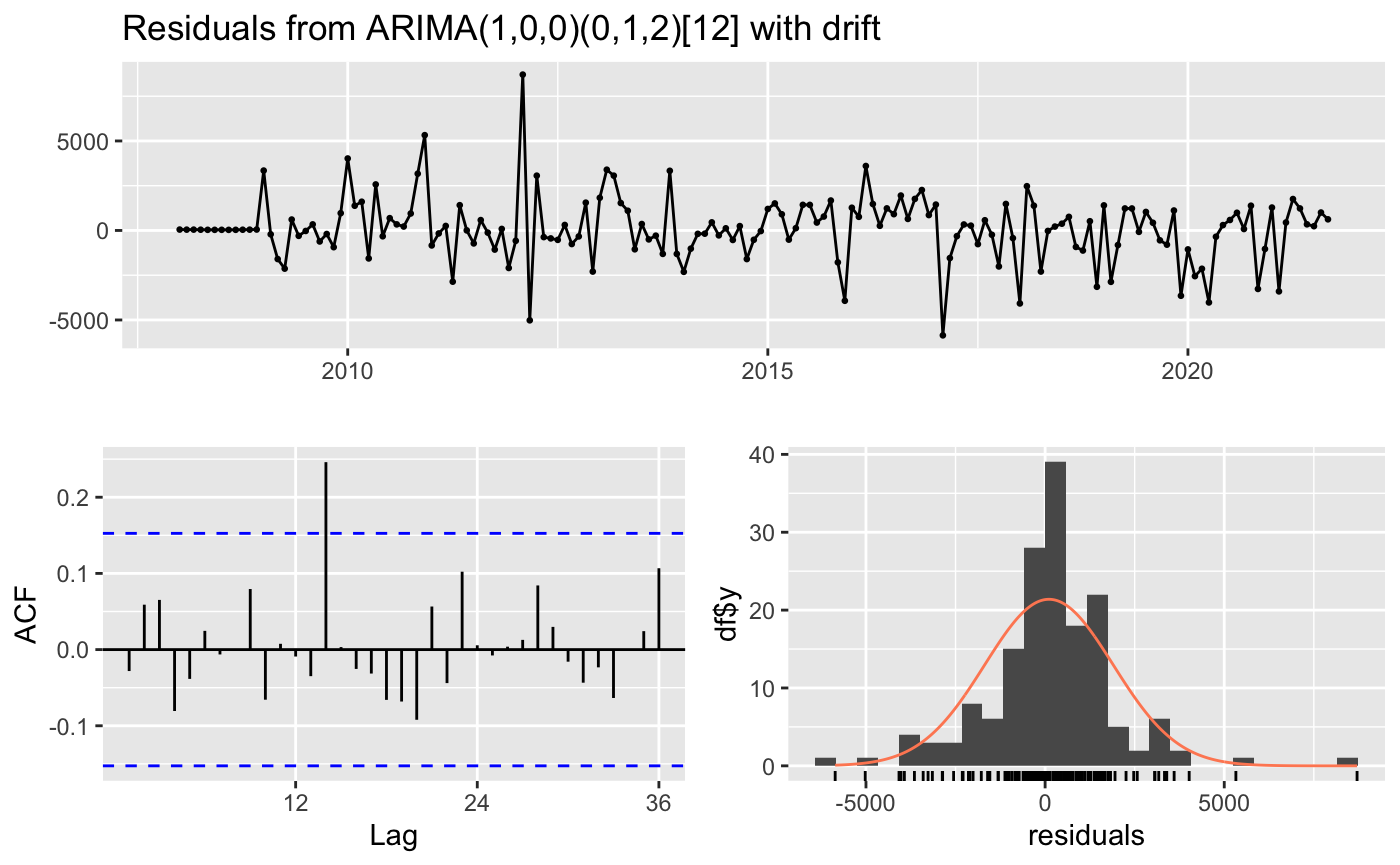
\includegraphics[width=1\linewidth]{images/residual_auto.png}
    \caption{Residuals Diagnostics ARIMA(1,0,0)(0,1,2)[12] (Auto.Arima)}
    \label{fig:residual_auto}
\end{figure}

\noindent\textbf{Residual Diagnostics}

To verify the adequacy of the fitted model, we performed diagnostic checks on the residuals, Fig.\ref{fig:residual_auto}. The diagnostic results showed the following:

\begin{itemize}
    \item The residuals plot reveals no discernible patterns and oscillates around a zero mean.
    \item The ACF of the residuals presents only one significant spike, suggesting minimal autocorrelation.
    \item The Ljung-Box test returns a high p-value (0.35), indicating no significant autocorrelation structure in the residuals.
\end{itemize}

These results confirm that the residuals behave like white noise, suggesting that the model captures the underlying structure of the training data effectively without patterns and non-autocorrelated.

\subsection{Manual SARIMA Model Specification}

As an alternative to automated model selection, we manually specified a SARIMA model based on analysis of the ACF and PACF plots of the stationary series. The chosen model \textbf{SARIMA(1,1,1)(0,1,1)[12]} reflects regular and seasonal differencing, both of which were deemed necessary from earlier transformation steps. We fitted the model to the training set using the \textit{arima()} function without including a drift term (as recommended when d = 1).

This alternative SARIMA model uses \( p = 1 \) and \( q = 1 \), values that were selected based on the non-seasonal lags of the ACF and PACF plots analyzed during the model identification phase.\\

\begin{itemize}
    \item \textbf{AR(1):} ar1=0.3651, significant (low standard error).
    \item \textbf{MA(1):} ma1=-0.9689, nearly -1, suggesting strong short-term smoothing.
    \item \textbf{Seasonal MA(1):} sma1=-1.0000, indicating strong seasonal dependence.
    \item \textbf{Standard error } = 0.1472, likely significant.
\end{itemize}

The estimated parameters are interpretable and appear to be statistically significant. When comparing information criteria to the previous automatic model \texttt{SARIMA(2,0,0)(0,1,2)[12]}, we observe that AIC, AICc, and BIC are lower, suggesting that the manual model achieves a better fit.\\

\noindent\textbf{Training Error Metrics}

\begin{itemize}
\item \textbf{ME:} -254.29 – small negative bias, suggesting slight underestimation.
\item \textbf{RMSE:} 1759.58 – relatively low magnitude of residual errors.
\item \textbf{MAPE:} 3.07\% – excellent accuracy (values below 10\% are typically acceptable).
\item \textbf{ACF1:} -0.028 – close to zero, indicating no residual autocorrelation.
\end{itemize}

\noindent\textbf{Residual Diagnostics}

We applied residual analysis to validate the adequacy of the model and the diagnostic plots show, Fig.\ref{fig:residual_manual}:

\begin{itemize}
    \item Residuals fluctuate randomly around zero with no visible structure.
    \item ACF of residuals shows one or two marginally significant spikes, but overall no meaningful autocorrelation.
    \item Ljung-Box test returns a p-value of 0.13, meaning we cannot reject the null hypothesis of independently distributed residuals.
\end{itemize}

\begin{figure}[H]
    \centering
    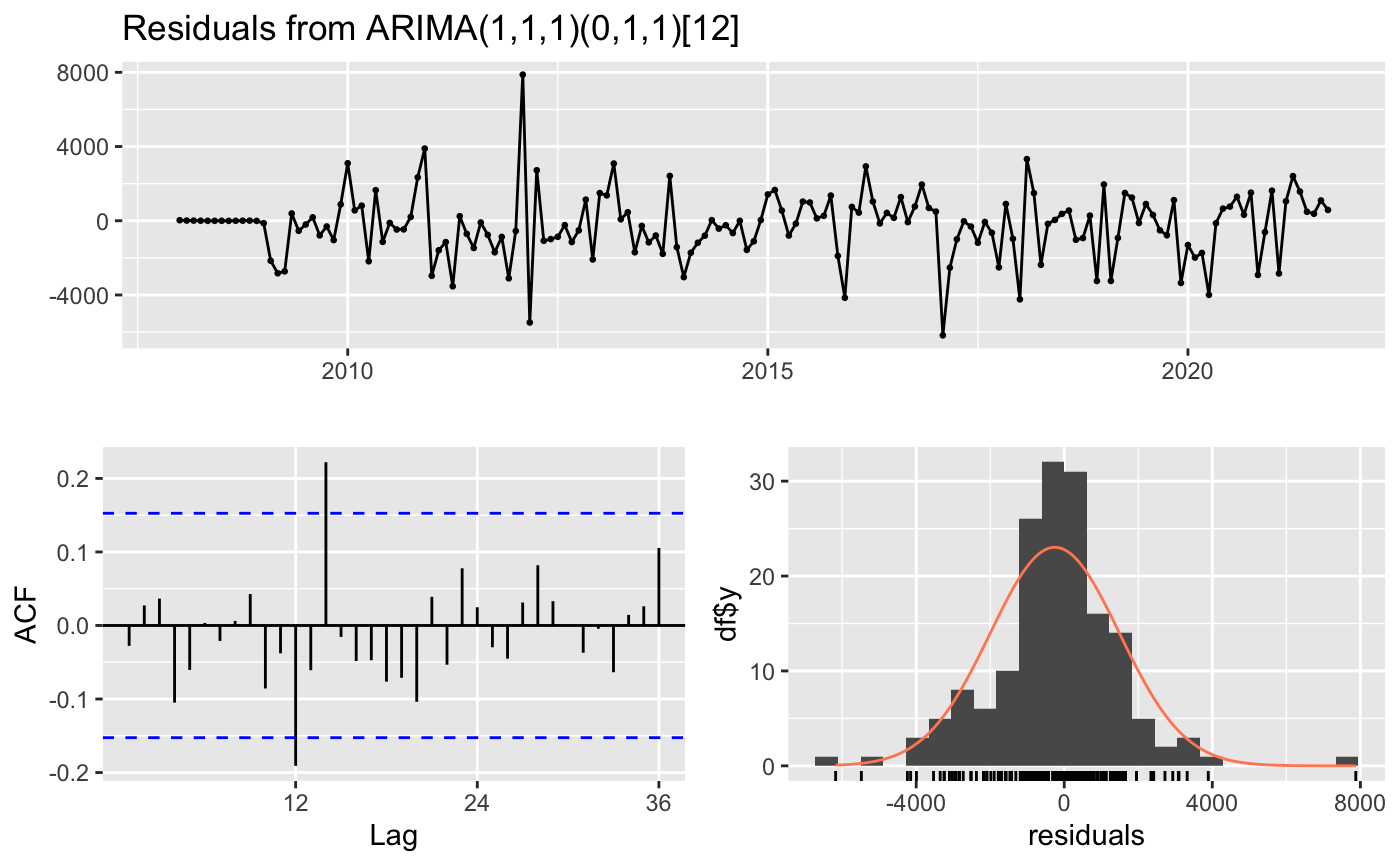
\includegraphics[width=1\linewidth]{images/manual_arima.png}
    \caption{Residuals Diagnostics SARIMA(1,1,1)(0,1,1)[12]}
    \label{fig:residual_manual}
\end{figure}


These results confirm that the model passes all diagnostic checks. The residuals behave like white noise, suggesting the model effectively captures the dynamics of the training series, similarly to the automatic SARIMA model.\\

\subsection{STL Decomposition Followed by ARIMA Modeling}

At this stage, we applied STL decomposition (seasonal-trend decomposition using loess), a technique that divides a time series into three components: trend, seasonality, and residuals. This makes it easier to model the residuals accurately, since the trend and seasonality have been removed. STL decomposition is particularly useful as it can be adjusted to be less sensitive to extreme values and more robust to outliers.\\

After decomposition, the residuals were modelled using an ARIMA model, which, in this case, fitted as an ARIMA(2, 1, 1). This strategy is effective in dealing with complexities or nonlinear variations in the seasonal components, enabling unstructured fluctuations to be modelled separately.\\

\begin{figure}[H]
    \centering
    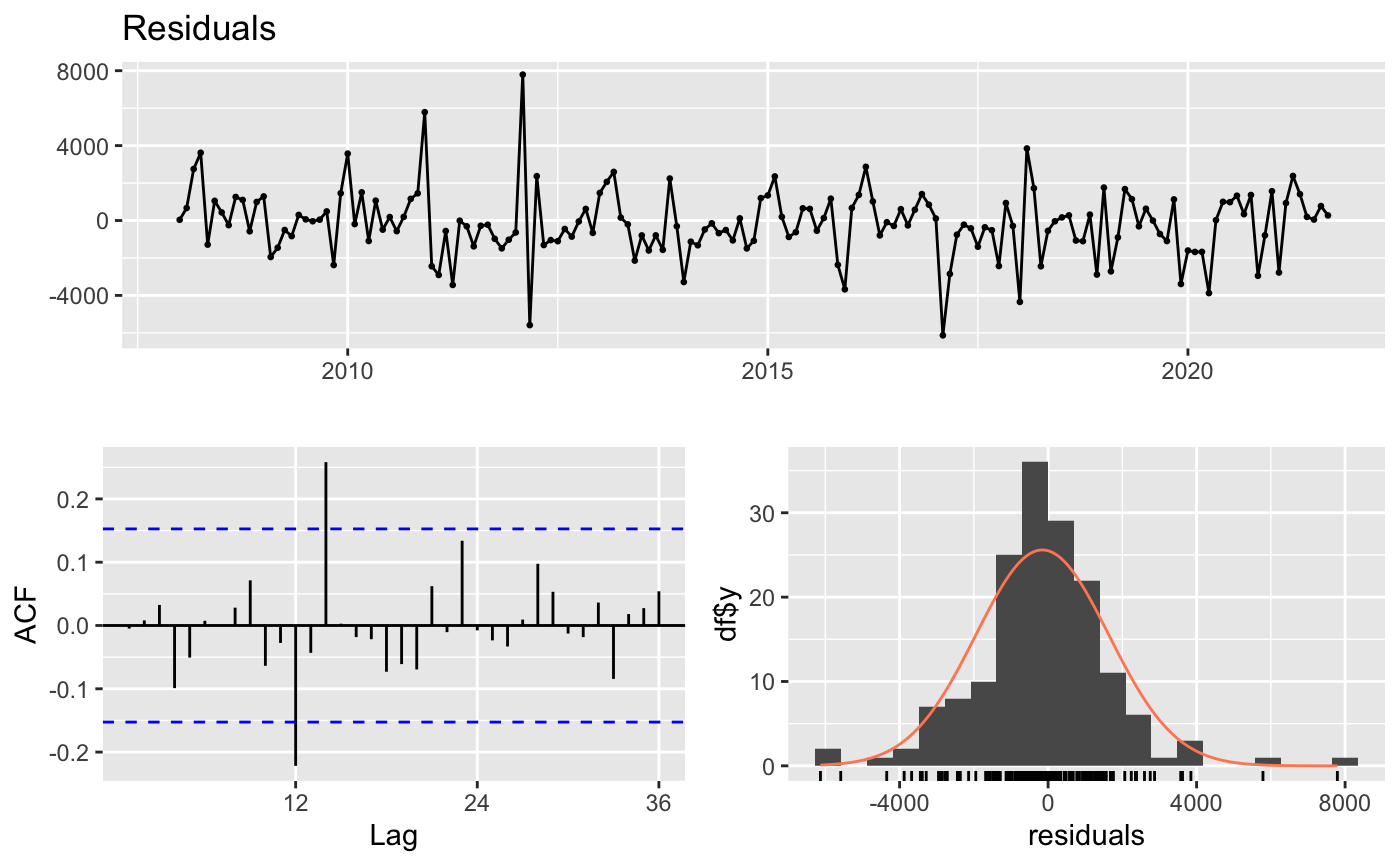
\includegraphics[width=1\linewidth]{images/st_red.png}
    \caption{Residuals Diagnostics STL decomposition with ARIMA(2,1,1)}
    \label{fig:st_red}
\end{figure}

 \noindent\textbf{Residual Diagnostics}

Analysis of the residuals from the STL + ARIMA model indicated that, Fig.\ref{fig:st_red}:
\begin{itemize}
    \item The residuals show no obvious patterns, oscillating randomly around zero.
    \item The autocorrelation function (ACF) of the residuals showed only a few isolated peaks, indicating that there is generally no significant correlation between the residuals.
    \item The Ljung–Box test showed a high p-value (0.11), implying that there is no evidence to reject the null hypothesis that the residuals are independent.
\end{itemize}

These results suggest that the model has successfully passed the diagnostic checks and that the residuals behave like white noise with no remaining systematic patterns or autocorrelation.

\subsection{Exponential Smoothing State Space Model (ETS)}

In this step, we fit an ETS model to the training data. The forecast package's \textit{ets()} function automatically selects the best model by testing various combinations of error, trend, and seasonality components (additive, multiplicative, and damped) and selecting the one with the lowest AICc value.

The ETS model is suitable for time series with systematic components, such as trends and seasonality, but with low noise. However, it does not address the issue of stationarity in the data, for which differentiation is recommended.

The selected model was ETS(M,Ad,M), which stands for:\\
- Error: Multiplicative (M)\\
- Trend: Additive Damped (Ad)\\
- Seasonality: Multiplicative (M)

This choice is consistent with the observed multiplicativity in the seasonality of the series, as well as incorporating a trend that amortises over time.\\

As for the smoothing parameters:\\
- Alpha (0.2592): a moderate value indicating a balance between the weight given to recent and past observations at series level.\\
- Gamma (1e-04) is practically zero, suggesting fixed seasonality over the period and low adaptability.

The seasonal vector shows variations over the 12-month cycle, with some months showing peaks, such as the winter months.

The sigma value (0.0445) indicates low residual variability, suggesting that the model reasonably well controls the residuals.\\

However, the information criteria (AIC and BIC) are considerably higher than those of previous models, suggesting that this model does not fit the series as well.
The residual autocorrelation (ACF1 approximatly 0.16) suggests that the residuals are slightly dependent. In addition, the model tends to underestimate the values, as indicated by the negative mean errors (ME and MPE).

This poorer fit can be explained by the non-stationarity of the data, which requires differentiation to stabilise the series, a transformation that the ETS model does not perform, thus compromising its fit.\\

\begin{figure}[H]
    \centering
    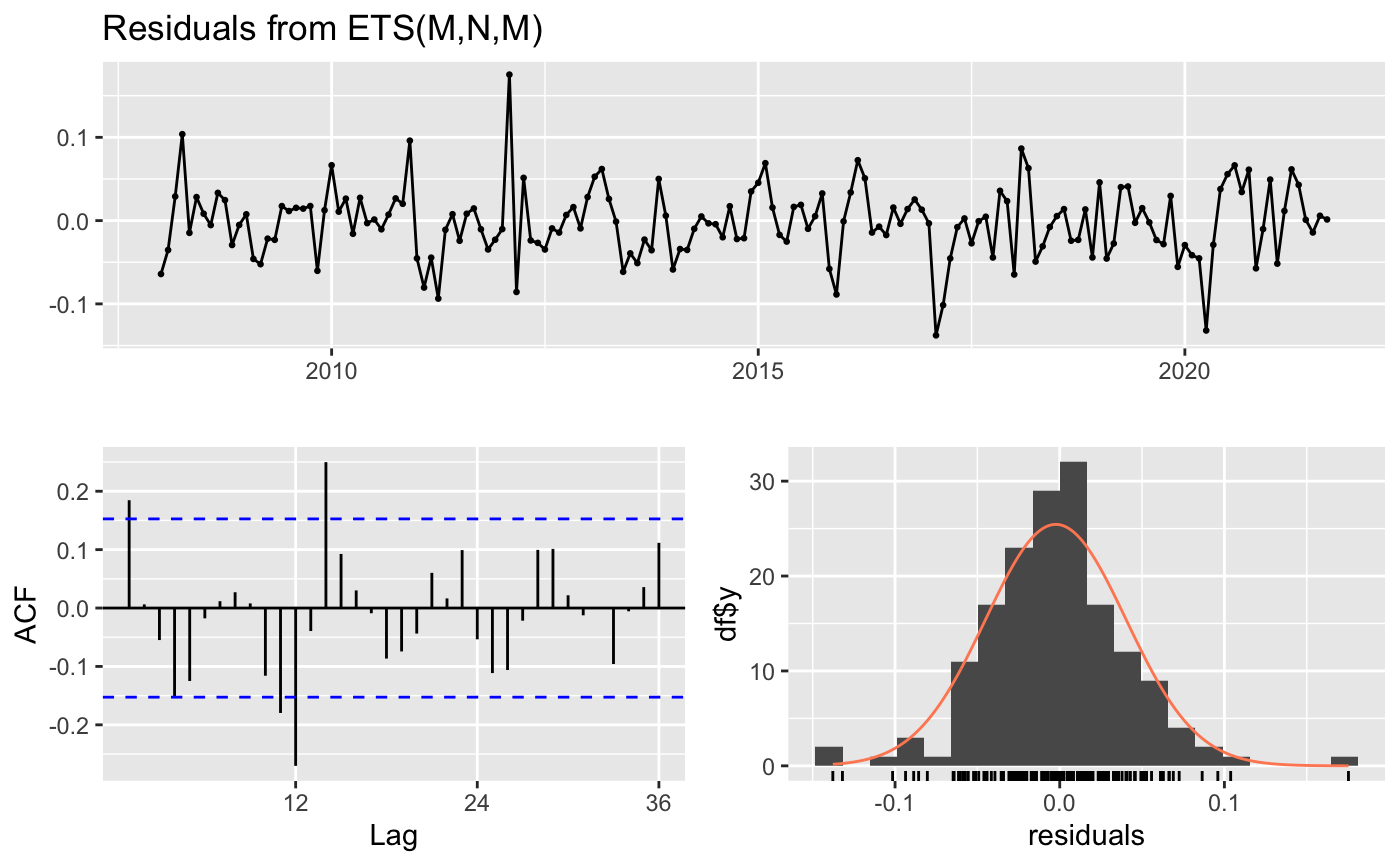
\includegraphics[width=1\linewidth]{images/ets_res.png}
    \caption{Residuals Diagnostics ETS(M,Ad,M)}
    \label{fig:res_ets}
\end{figure}

\noindent\textbf{Residual Diagnostics}

The graph of the residuals, Fig.\ref{fig:res_ets} shows random behaviour around zero, with no clear patterns.
The autocorrelation function of the residuals shows significant peaks, indicating residual correlation and the Ljung–Box test rejects the null hypothesis of residual independence, indicating that the residuals do not behave like white noise.

Therefore, the ETS model did not pass the diagnostic tests satisfactorily, as the residuals show significant autocorrelation, suggesting that patterns remain that the model has not captured.
\section{Forecast Evaluation and Confidence Analysis}

This section presents a detailed evaluation of the future observations forecasts for each of the statistical time series models developed: the Automatic SARIMA model, the Manual SARIMA model, the STL Decomposition followed by ARIMA Modeling (STLM), and the Exponential Smoothing State Space Model (ETS). For each model, we analyze the visual representation of the forecast against actual data, interpret the associated confidence intervals, and the accuracy values.

\subsection{Automatic SARIMA Model}

The SARIMA(2,0,0)(0,1,2)[12] model, automatically selected, was utilized to forecast the next 41 observations, covering the entire test set period. \\

\begin{figure}[H]
    \centering
    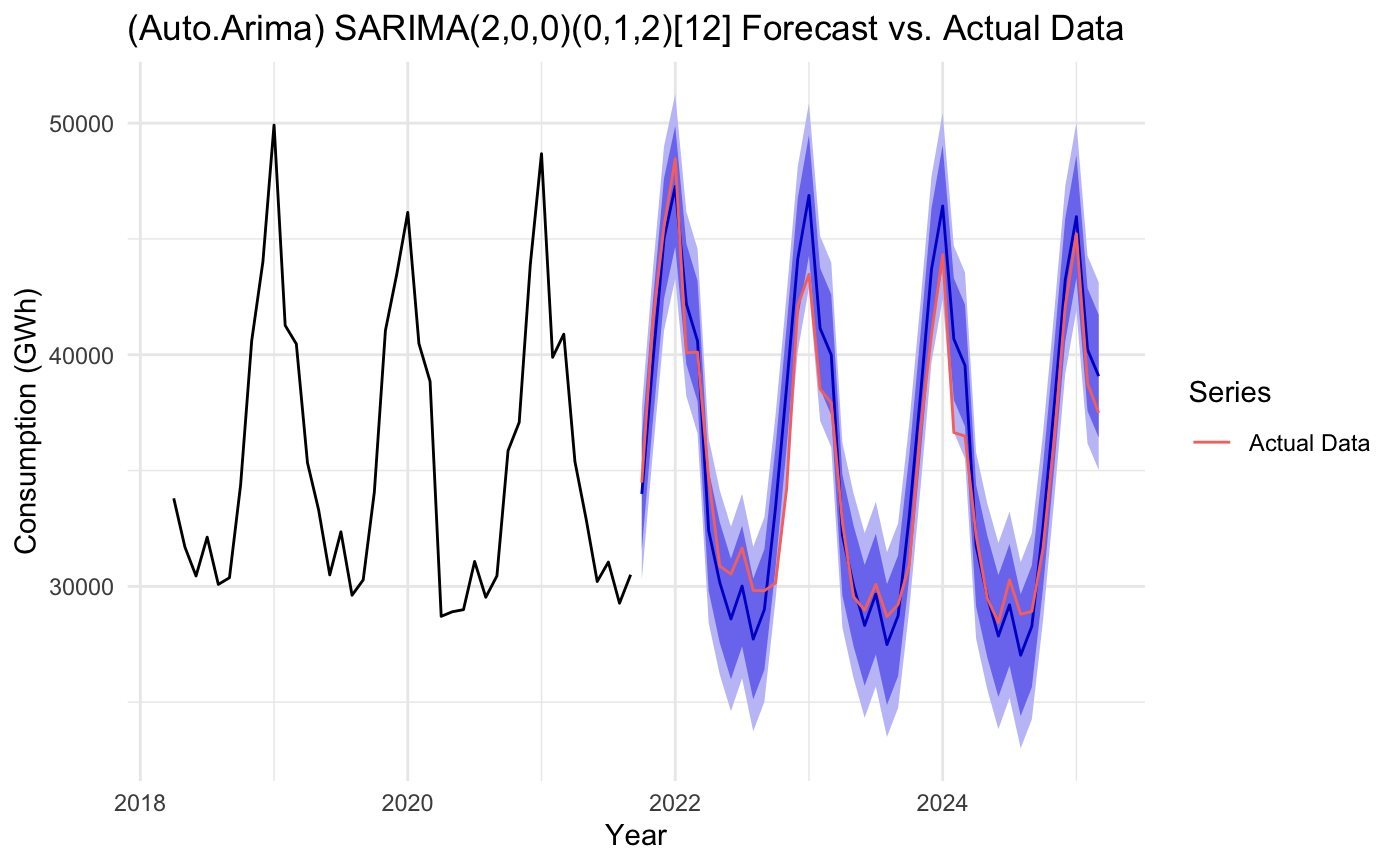
\includegraphics[width=1\linewidth]{images/for_auto.png}
    \caption{(Auto.Arima) SARIMA(2,0,0)(0,1,2)[12] Forecast vs. Actual Data}
    \label{fig:enter-label}
\end{figure}

The forecast plot for the Automatic SARIMA model shows strong performance over time. The forecast is accompanied by blue-shaded bands representing uncertainty levels: a darker band indicates higher confidence (95\%), while a lighter band denotes lower confidence (80\%). Crucially, most of the observed values (represented by the red line) fall within the 95\% confidence intervals. This indicates that the model is highly effective at capturing both the underlying trend and the variability of the electricity consumption series. Furthermore, the model accurately reproduces the regular seasonal patterns, with the confidence intervals successfully encompassing the extremes of the historical data, demonstrating a good fit to the seasonality. The gradual widening of these bands over time is an expected characteristic of time series forecasting, reflecting the increasing uncertainty in longer-term predictions.\\

Regarding forecast accuracy, the Mean Absolute Percentage Error (MAPE) on the test set was 4.37\%. This signifies that, on average, the model's forecasts deviated from the actual values by approximately 4.5\%. This is considered a high level of accuracy. The Root Mean Squared Error (RMSE) provides a measure of the typical error magnitude in Gigawatt-hours (GWh). The Theil's U statistic for the test set was 0.518, which is less than 1, confirming that this model outperforms a simple naive forecasting approach. While improved from the training set, the autocorrelation function at lag 1 (ACF1) of 0.619 on the test set suggests that some residual autocorrelation remains, implying that there might still be uncaptured patterns in the error term.\\

\subsection{Manual SARIMA Model}

The manually configured SARIMA(1,1,1)(0,1,1)[12] model was also used to generate forecasts, which were subsequently evaluated against the actual values within the test set.\\

\begin{figure}[H]
    \centering
    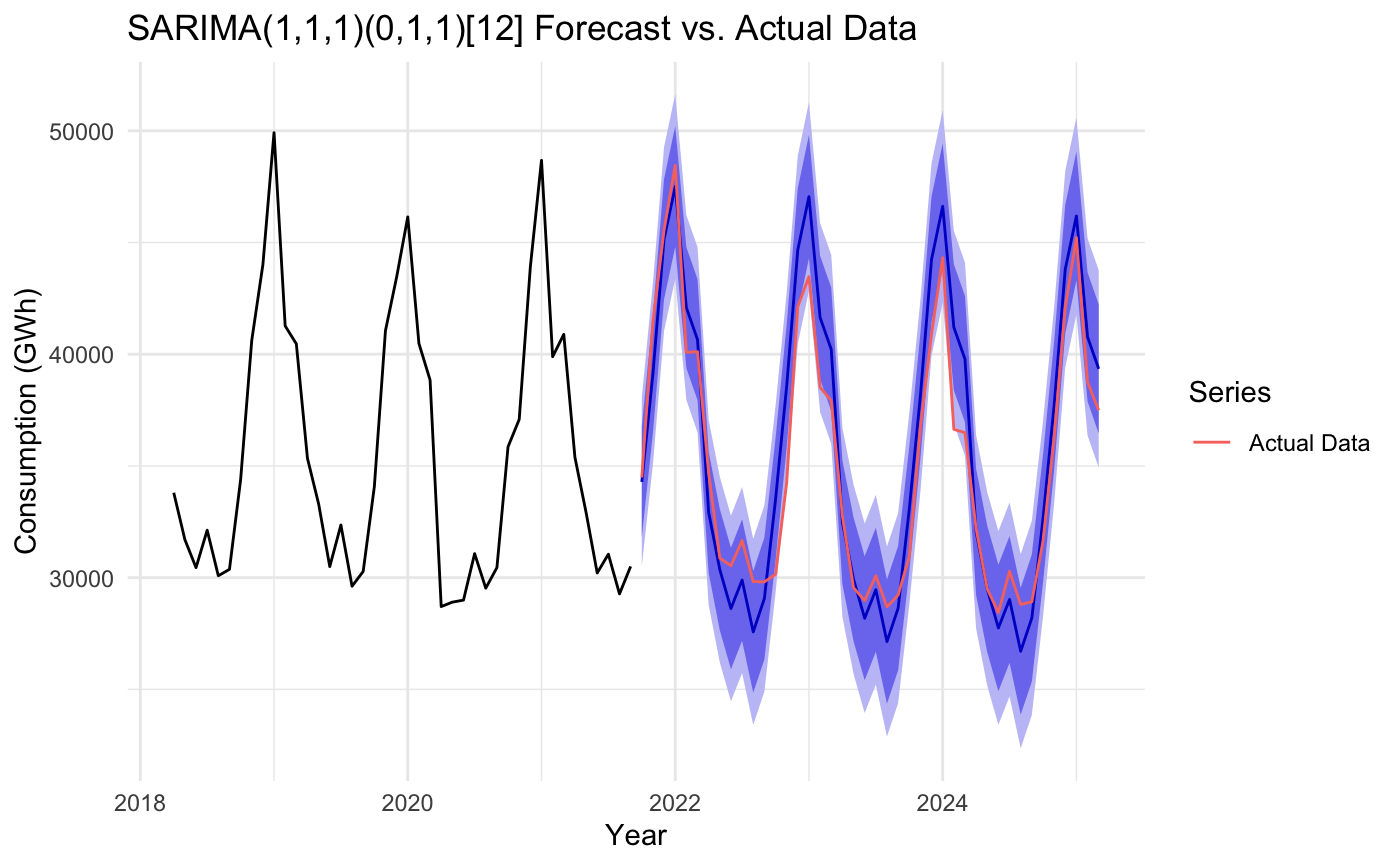
\includegraphics[width=1\linewidth]{images/for_ma.png}
    \caption{SARIMA(1,1,1)(0,1,1)[12] Forecast vs. Actual Data}
    \label{fig:enter-label}
\end{figure}

Similar to the automatically selected SARIMA model, the manually configured SARIMA forecast also exhibited good performance when compared to the actual data. The confidence bands, represented by blue shading, follow the same interpretation as before: darker shades indicate higher confidence (95\%), and lighter shades indicate lower confidence (80\%). The majority of the actual values (red line) remained within the 95\% confidence intervals, suggesting that the model effectively captured the trend and variability of the series throughout the forecast period. The seasonal patterns observed in the actual data were well replicated by the model, further indicating a good fit to the series' seasonality. The widening of the confidence bands over time is a typical and expected behavior in time series models, reflecting increasing uncertainty as the forecast horizon extends.\\

In terms of forecast accuracy, the Mean Absolute Percentage Error (MAPE) on the test set was 4.67\%. This remains a very good value, demonstrating a high level of accuracy. The Theil's U statistic of 0.558 (below 1) validates the model's predictive utility by confirming its outperformance of a naive prediction. While absolute and percentage errors naturally increased on the test set compared to the training set, they remained at acceptable levels. However, a notable increase in the autocorrelation of the residuals (ACF1 = 0.657) was observed on the test set. This suggests that the model might not have fully captured all underlying patterns in the future data, implying that exploring other SARIMA orders could potentially lead to further improvements.\\

\subsection{STL Decomposition Followed by ARIMA Modeling}

The STL + ARIMA(2,1,1) model, which first decomposes the time series and then applies ARIMA to the remainder, was assessed for its future forecasts.\\

\begin{figure}[H]
    \centering
    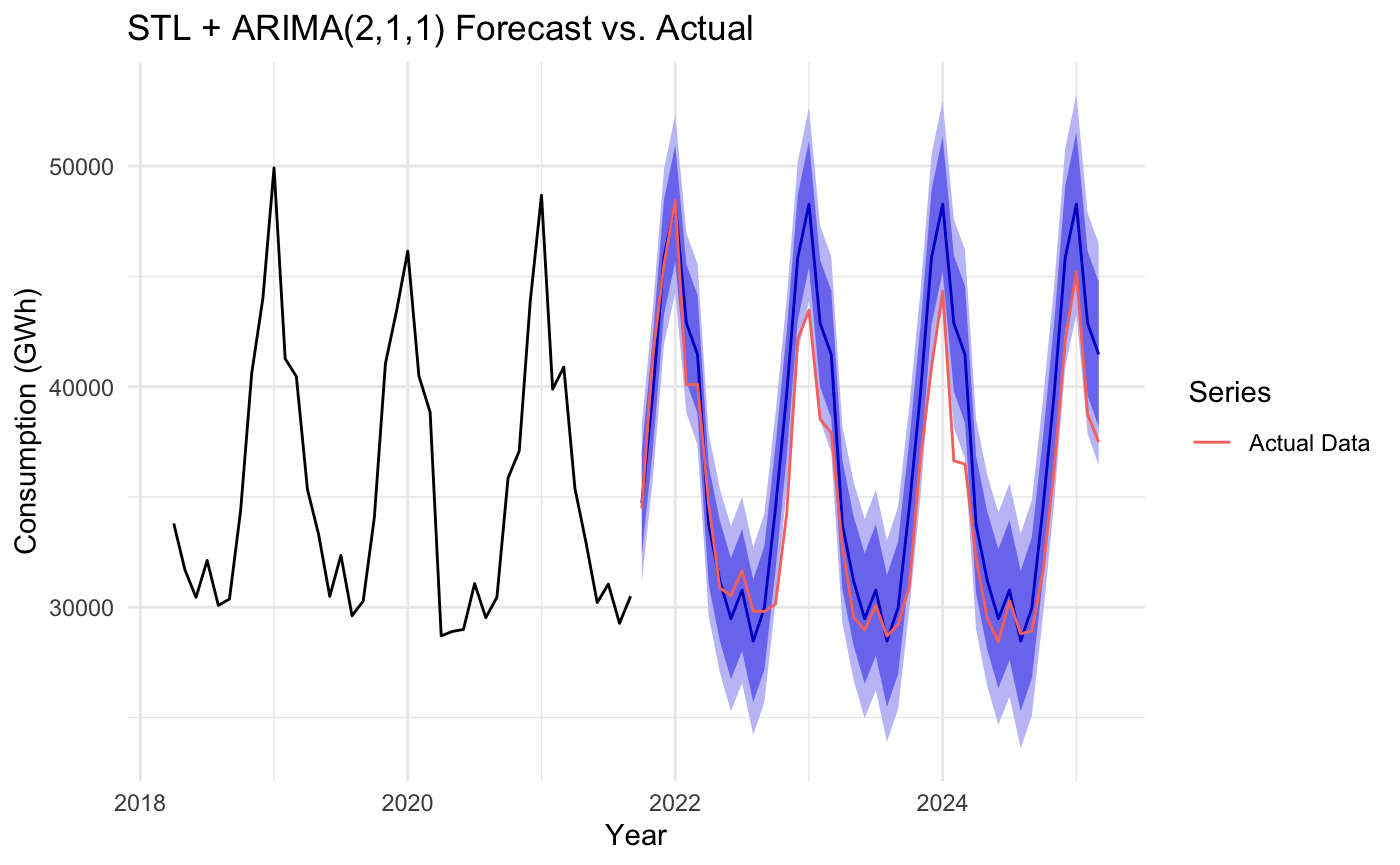
\includegraphics[width=1\linewidth]{images/for_stml.png}
    \caption{STL + ARIMA(2,1,1) Forecast vs. Actual}
    \label{fig:enter-label}
\end{figure}

The forecast generated by the STL + ARIMA(2,1,1) model showed satisfactory results over time. The confidence bands, indicating uncertainty, were present and interpreted similarly to the SARIMA models. While the actual values (red line) largely remained within the 95\% confidence intervals, unlike the SARIMA models, there were instances where they only fell within the 80\% range or even outside the intervals. Nevertheless, the model generally managed to capture the trend and variability of the time series well for most of the forecast horizon. The seasonal patterns inherent in the data were adequately represented, reflecting the effectiveness of the seasonal decomposition performed by the STL method. The expected widening of the confidence bands over time confirmed the natural increase in uncertainty for more distant forecast periods.\\

For forecast accuracy, the model exhibited good training performance, with training residuals closely resembling white noise (ACF1 $\approx$ 0) and a MASE (Mean Absolute Scaled Error) less than 1, along with a MAPE of approximately 3\%. This indicates strong in-sample performance. However, a significant deterioration in performance was observed on the test set, with all error metrics increasing substantially ($MAPE > 6\% $ and  $MASE > 1$). The high ACF1 of 0.69 on the test set points to strong autocorrelation in the errors, suggesting underfitting to the most recent data. This indicates that the model might not have captured new patterns or recent structural changes specific to the test period, or that the chosen ARIMA order for the residuals was inappropriate, leading to out-of-sample underfitting. The Theil's U value of 0.779 suggests it still performs better than a naive forecast, but less effectively than the SARIMA models.\\

\subsection{Exponential Smoothing State Space Model (ETS)}

The ETS model was employed to generate forecasts for future electricity consumption.\\

\begin{figure}[H]
    \centering
    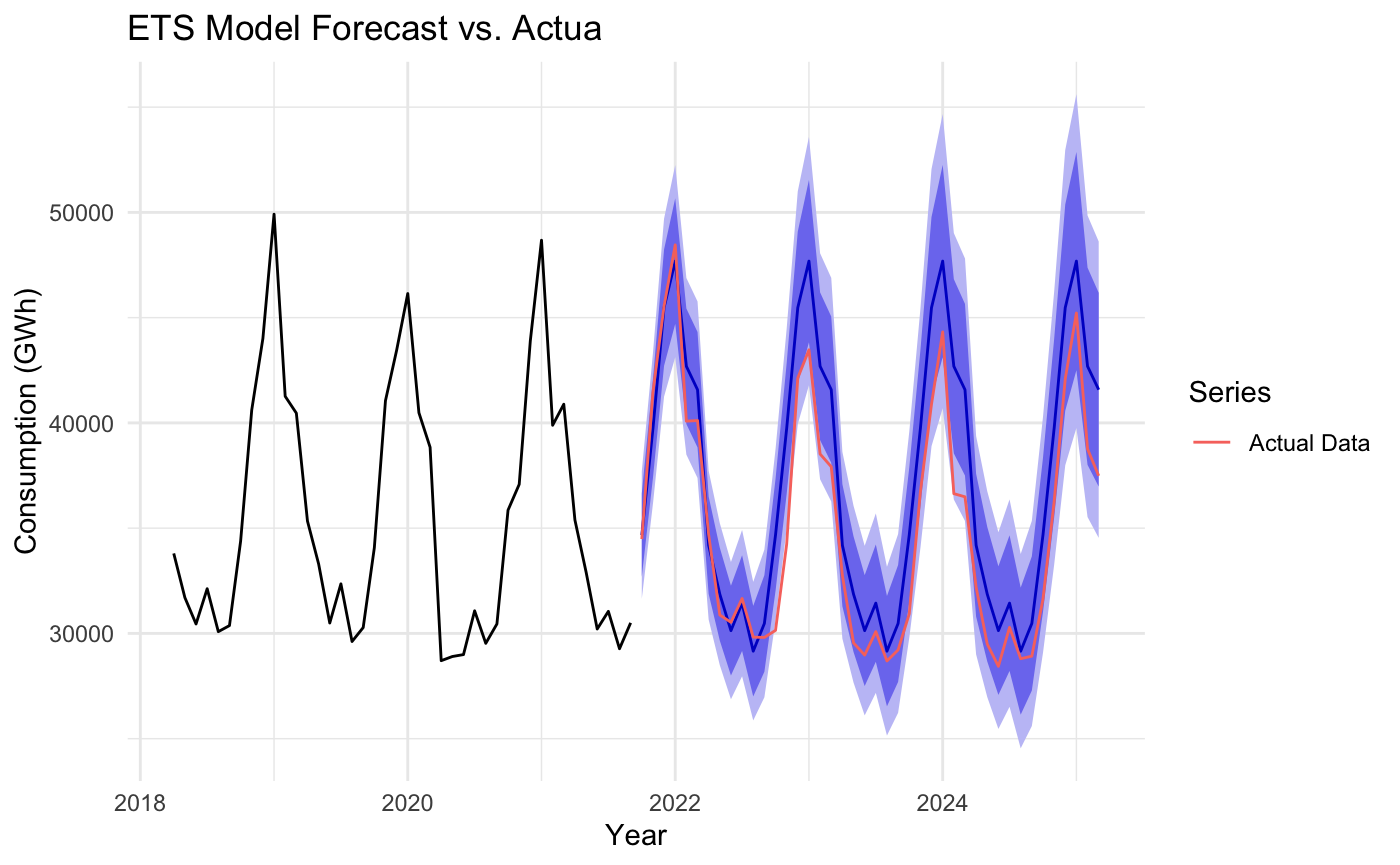
\includegraphics[width=1\linewidth]{images/for_ets.png}
    \caption{ETS Model Forecast vs. Actual}
    \label{fig:enter-label}
\end{figure}

Similar to the SARIMA models, the ETS forecast also showed good results over time. The blue-shaded bands represented the familiar uncertainty levels (95\% and 80\% confidence). Most of the observed values (red line) stayed within the 95\% confidence intervals, indicating that the model effectively captured both the trend and variability of the series. The regular seasonal patterns were well-represented, with the intervals successfully capturing the extremes of the historical series, suggesting a good fit to the seasonality. The widening of the confidence bands over time, reflecting increasing uncertainty for longer-term forecasts, was also an expected behavior.\\

In terms of forecast accuracy, on the training set, the model fit well with relatively low error rates (MAPE $\approx$ 3.2\%) and better performance than the naive model ($MASE < 1)$. However, on the test set, errors increased significantly ($MAPE > 6\%$, $MASE > 1$), pointing to poorer out-of-sample performance. Additionally, the high residual autocorrelation on the test set (ACF1 $\approx$ 0.65) suggests that the model did not fully capture all the series' patterns, possibly due to underfitting or shifts in the data's underlying dynamics. The Theil's U value of 0.787 confirms that the ETS model performs better than a naive forecast, but its performance on the test set is notably weaker compared to both SARIMA models.\\



\section{Results and Discussion}

This section presents a comprehensive analysis of our model evaluation results about the most effective approach for forecasting monthly electricity consumption in France. We examine detailed accuracy metrics and visual diagnostics for each statistical time series model — the Automatic SARIMA, Manual SARIMA, STL Decomposition followed by ARIMA (STLM), and Exponential Smoothing State Space Model (ETS) — to identify the model that delivers the most reliable and robust forecasts.

\subsection{Model Comparison Based on Information Criteria}


In addition to error metrics, information criteria such as AIC (Akaike Information Criterion), AICc (corrected AIC) and BIC (Bayesian Information Criterion) are fundamental to assessing model fit, considering adherence to the data and model complexity.

These criteria penalise overly complex models and help avoid overfitting. They are particularly useful for comparing models fitted to the same set of data.

\begin{figure}[H]
    \centering
    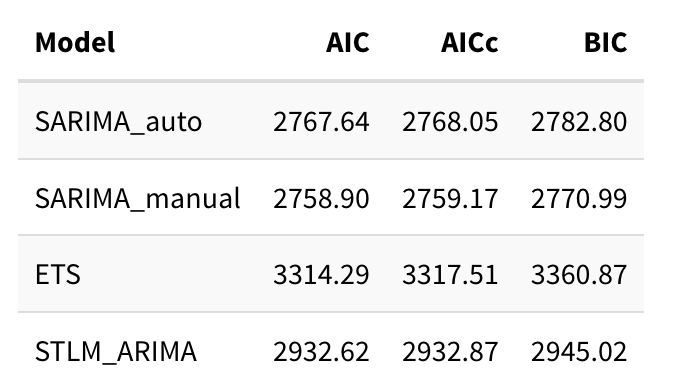
\includegraphics[width=0.75\linewidth]{images/table1.png}
    \caption{Comparison of Information Criteria across Models}
    \label{fig:enter-label}
\end{figure}

When the AIC, AICc and BIC criteria are compared between the models, it can be seen that the SARIMA\_manual model has the lowest values for all metrics, indicating a better balance between fit and model complexity. The SARIMA\_auto model performed similarly, but slightly less well. In contrast, the STLM\_ARIMA and ETS models had significantly higher values, suggesting that they fit the data less efficiently, possibly due to greater complexity or an inability to capture the patterns in the series. Therefore, based on the information criteria, the SARIMA\_manual model is the most suitable for this time series.

\subsection{Model Comparison Based on Forecast Accuracy}
To evaluate the predictive ability of the various models, we examined the error metrics in the test set. The metrics considered were RMSE (root mean squared error), MAE (mean absolute error), MAPE (mean absolute percentage error) and Theil's U. These metrics provide different perspectives on the quality of the forecasts.

The table below summarises these metrics for the four evaluated models: SARIMA with automatic parameter selection (SARIMA\_auto); SARIMA with manual parameters (SARIMA\_manual); the ETS model; and the hybrid STLM model with ARIMA in the residuals (STLM\_ARIMA). The aim of this comparison is to identify the model with the best predictive performance and the lowest error in forecasting future values of the series.

\begin{figure}[H]
    \centering
    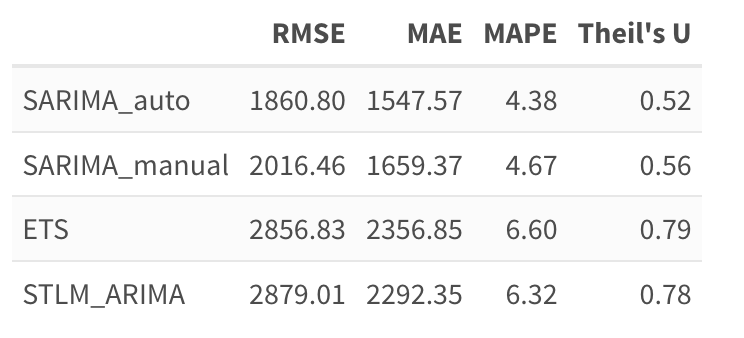
\includegraphics[width=0.75\linewidth]{images/table2.png}
    \caption{Forecast Accuracy Comparison on Test Set}
    \label{fig:enter-label}
\end{figure}

When the models were compared based on the forecasting metrics in the test set, the SARIMA\_auto model exhibited the best overall performance, showing the lowest RMSE, MAE, MAPE and Theil's U values. This indicates greater accuracy and better predictive capacity. SARIMA\_manual performed reasonably well, albeit slightly less well than the automatic model. The ETS and STLM\_ARIMA models, on the other hand, produced significantly higher error values, suggesting that they are less effective for forecasting this series. Therefore, the automatic SARIMA model is the most suitable choice for future forecasting.

\subsubsection{Forecast Visualisation}
In addition to quantitative metrics, visually comparing the predictions with the actual data is fundamental to understanding how each model behaves over time. The graph below shows the actual values of the test set alongside the forecasts generated by each model.

This visualisation enables us to identify any systematic deviations, as well as the models' ability to capture seasonality and trends, and any delays or one-off errors in the forecasts.

By comparing the model forecasts with the actual data, we conclude that SARIMA\_auto and SARIMA\_manual produced the most accurate predictions.

\begin{figure}[H]
    \centering
    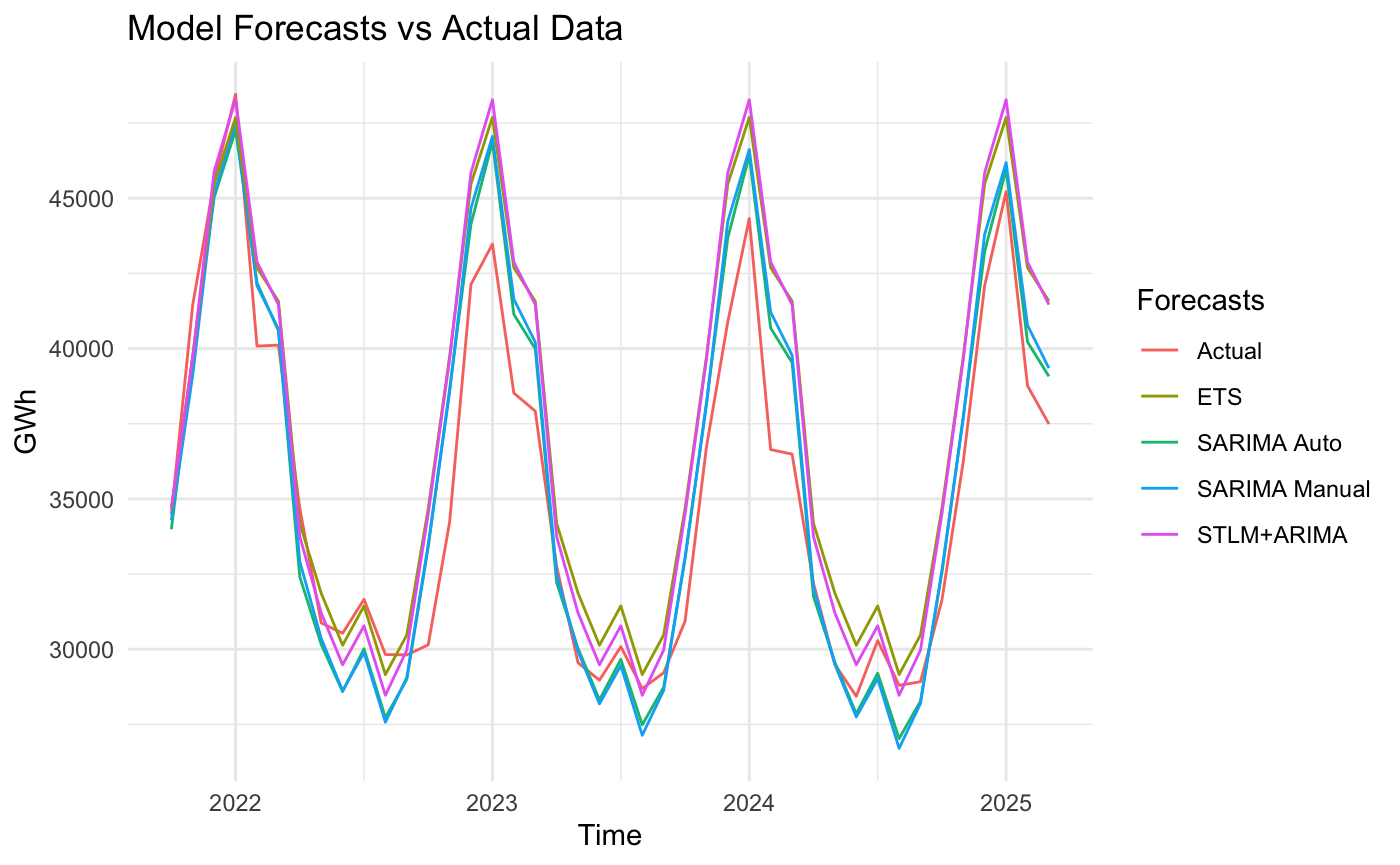
\includegraphics[width=1\linewidth]{images/grafico_fixe.png}
    \caption{Forecast Visualisation of the four models}
    \label{fig:enter-label}
\end{figure}

\section{Conclusion}
When analysing the information criteria (AIC, AICc and BIC) and forecast accuracy metrics (RMSE, MAE, MAPE and Theil's U) in the test set, the SARIMA\_auto and SARIMA\_manual models emerged as the most suitable for modelling the time series.

SARIMA\_manual produced the lowest information criterion values, indicating the best balance between model fit and complexity. However, SARIMA\_auto obtained the lowest forecast errors in terms of predictive performance, suggesting greater capacity for generalisation and accuracy in future data.

Conversely, the ETS and STLM\_ARIMA models exhibited significantly higher values in both the information criteria and the error metrics, suggesting poorer model fit and forecasting performance.

Therefore, the ideal choice depends on the objective: SARIMA\_manual is more suitable for better historical adjustment, while SARIMA\_auto is superior for future forecasting with lower error. Overall, SARIMA models are more appropriate for this data than ETS and STLM\_ARIMA models. By comparing the models' forecasts with the actual data, we can conclude that SARIMA\_auto and SARIMA\_manual produced the most accurate predictions.

% printing acronyms
\printglossary[type=\acronymtype,title=Acronyms]

% references section
\bibliography{refs}
\bibliographystyle{IEEEtran}

\section{Appendix}
\end{document}